\subsection*{Problema 31}
\noindent\textbf{Enunciado:} Calcular la integral:
\begin{equation*}
\int \dfrac{x^2 \, dx}{(4 + x^3)^{1/2}}
\end{equation*}

\noindent\textbf{Solución:}
Para resolver la integral dada, empleamos el método de sustitución. 
Identificamos la función interna en el denominador y definimos la nueva variable $u$:
\begin{equation*}
u = 4 + x^3
\end{equation*}

Calculamos la diferencial $du$:
\begin{align*}
du &= \dfrac{d}{dx}(4 + x^3) \, dx \\
du &= 3x^2 \, dx
\end{align*}

Despejamos el término $x^2 \, dx$ para que coincida exactamente con el numerador del integrando:
\begin{equation*}
x^2 \, dx = \dfrac{1}{3} \, du
\end{equation*}

Sustituimos la variable $u$ y su diferencial en la integral original:
\begin{align*}
\int \dfrac{x^2 \, dx}{(4 + x^3)^{1/2}} &= \int \dfrac{\frac{1}{3} \, du}{u^{1/2}} \\
&= \dfrac{1}{3} \int u^{-1/2} \, du
\end{align*}

Aplicamos la regla de integración para potencias, $\int u^n \, du = \frac{u^{n+1}}{n+1}$:
\begin{align*}
\dfrac{1}{3} \int u^{-1/2} \, du &= \dfrac{1}{3} \left( \dfrac{u^{1/2}}{\frac{1}{2}} \right) + C \\
&= \dfrac{2}{3} u^{1/2} + C
\end{align*}

Finalmente, regresamos a la variable original $x$ sustituyendo $u = 4 + x^3$:
\begin{equation*}
\int \dfrac{x^2 \, dx}{(4 + x^3)^{1/2}} = \dfrac{2}{3}(4 + x^3)^{1/2} + C
\end{equation*}

\begin{figure}[H]
	\centering
	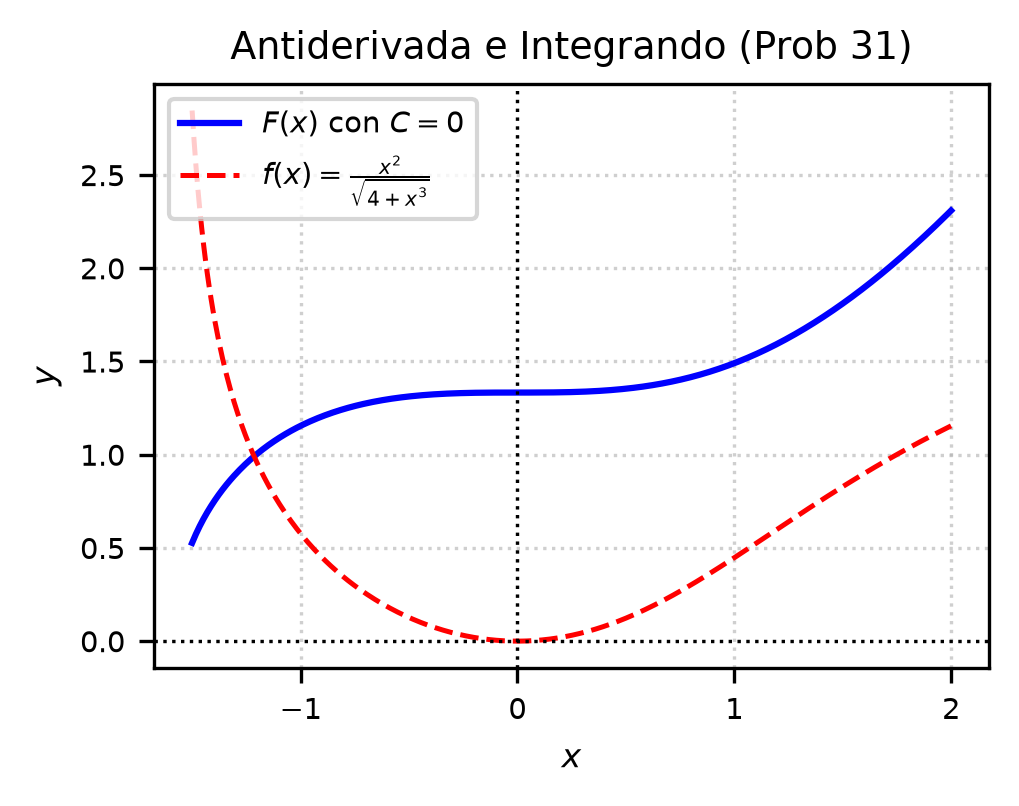
\includegraphics[width=\columnwidth]{semana_05/graficas/SEM05_P31_grafica.png}
	\caption{Representación gráfica de $f(x)$ y su antiderivada $F(x)$ evaluada para la constante de integración $C = 0$ (Problema 31).}
	\label{fig:problema31}
\end{figure}
